\mySection{Experimental Results}

\subsection{Accuracy of Facial Recognition}
In our experiments, we select a variable n $\in$ $\{5, 10, 15, 20, 25, 30\}$ as our experimental parameter,
where n is the number of facial embeddings pre-computed per person. Simply put, n is the
number of photos collected from each individual before actually performing facial recognition.
Each time the experiment yields the number of faces recognized correctly, denoted by p.
We define another variable k to represent the number of faces in a testing set.
Finally, the correct rate $C_n$  for an experiment with respect to the parameter n can be evaluated by equation~\ref{eq:correct-rate}.

\begin{equation}
  \label{eq:correct-rate}
  C_n = p / k
\end{equation}

To assess how well our system can recognize faces with respect to different values of n,
i.e., with different numbers of photos collected in advance from each person, we perform an experiment
6 times on each testing set. Moreover, since we have three testing sets, we perform the experiment
18 times in total. All values of $C_n$ collected from our experiments are presented in table~\ref{tab:exp-result-tab}.
the visualization of which is shown in figure~\ref{fig:exp-result-chart}.
The results indicate that PyRollCall can achieve approximately \textbf{70\% to 85\%} of correct rate
for facial recognition at its best if \textbf{25 to 30} photos are collected in advance from each individual.
\vspace{0.5cm}

\begin{table}[!htb]
\centering
\caption{Correct rates for PyRollCall's facial recognition feature.} 
\begin{tabular}{@{}lcccccc@{}}
\toprule[2pt]
& \multicolumn{6}{c}{Number of embeddings pre-computed per person}                                                                                                                              \\ \addlinespace[0.5em]
                  & 5                          & 10                         & 15                         & 20                         & 25                         & 30                         \\ \midrule \addlinespace[0.5em]
Testing Set 1     & 8/20                       & 10/20                      & 15/20                      & 17/20                      & 17/20                      & 17/20                      \\
                  & \multicolumn{1}{c}{(40\%)} & \multicolumn{1}{c}{(50\%)} & \multicolumn{1}{c}{(75\%)} & \multicolumn{1}{c}{(85\%)} & \multicolumn{1}{c}{(85\%)} & \multicolumn{1}{c}{(85\%)} \\ \addlinespace[0.5em] \midrule \addlinespace[0.5em]
Testing Set 2     & 8/20                       & 10/20                      & 12/20                      & 13/20                      & 14/20                      & 14/20                      \\
                  & \multicolumn{1}{c}{(40\%)} & \multicolumn{1}{c}{(50\%)} & \multicolumn{1}{c}{(60\%)} & \multicolumn{1}{c}{(65\%)} & \multicolumn{1}{c}{(70\%)} & \multicolumn{1}{c}{(70\%)} \\ \addlinespace[0.5em] \midrule \addlinespace[0.5em]
Testing Set 3     & 9/20                       & 13/20                      & 14/20                      & 15/20                      & 15/20                      & 15/20                      \\
                  & \multicolumn{1}{c}{(45\%)} & \multicolumn{1}{c}{(65\%)} & \multicolumn{1}{c}{(70\%)} & \multicolumn{1}{c}{(75\%)} & \multicolumn{1}{c}{(75\%)} & \multicolumn{1}{c}{(75\%)} \\ \addlinespace[0.5em] \midrule[2pt] \addlinespace[0.5em]
Avg. Correct Rate & 41.67\%                    & 55\%                       & 68.33\%                    & 75\%                       & 76.67\%                    & 76.67\%                    \\ \addlinespace[0.5em]
\bottomrule[2pt]
\end{tabular}
\label{tab:exp-result-tab}
\end{table}
\vspace{0.2cm}

\begin{figure}[!htb]
  \centering
  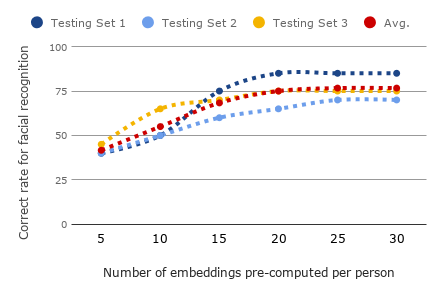
\includegraphics[width=0.8\linewidth]{figures/exp-result-chart.png}
  \caption{Visualization of the correct rates for PyRollCall's facial recognition feature.}
  \label{fig:exp-result-chart}
\end{figure}
\clearpage


\subsection{Analysis of Correct Facial Recognition}


\subsection{Analysis of Faulty Facial Recognition}
In most cases, PyRollCall can recognize faces correctly as long as 25 to 30 photos are collected
beforehand from each individual. However, sometimes erroneous facial recognition can still take place,
especially if the targets are wearing makeup. Figure~\ref{fig:false-recog1} shows an example where
faulty facial recognition happens due to makeup.
\vspace{0.2cm}

\begin{figure}[!htb]
  \centering
  \begin{subfigure}[b]{0.3\linewidth}
    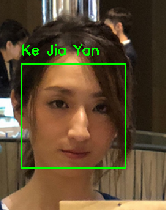
\includegraphics[width=\linewidth]{figures/false-recog-correct1.png}
    \caption{Ke Jia Yan}
  \end{subfigure}
  \begin{subfigure}[b]{0.3\linewidth}
    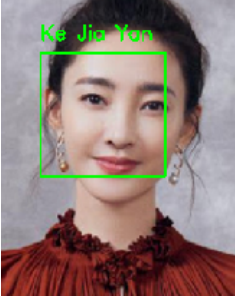
\includegraphics[width=\linewidth]{figures/false-recog-error1.png}
    \caption{Wang Li Kun}
  \end{subfigure}
  \caption{Erroneous facial recognition, example 1.}
  \label{fig:false-recog1}
\end{figure}


Another reason which can lead to error in facial recognition is insufficient amount of photos collected,
as shown in figure~\ref{fig:false-recog2}. Even with 30 photos collected for each individual in advance,
sometimes the result can still be faulty.
\vspace{0.2cm}

\begin{figure}[!htb]
  \centering
  \begin{subfigure}[b]{0.3\linewidth}
    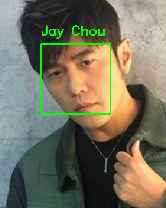
\includegraphics[width=\linewidth]{figures/false-recog-correct2.png}
    \caption{Jay Chou}
  \end{subfigure}
  \begin{subfigure}[b]{0.3\linewidth}
    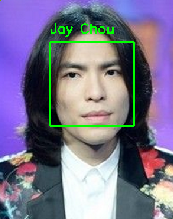
\includegraphics[width=\linewidth]{figures/false-recog-error2.png}
    \caption{Jam Hsiao}
  \end{subfigure}
  \caption{Erroneous facial recognition, example 2.}
  \label{fig:false-recog2}
\end{figure}
\vspace{0.5cm}


\subsection{Analysis of Correct Facial Recognition}
Next, we
With sufficient photos of students provided and their facial embeddings pre-computed,
the system will be able to detect and recognize faces correctly. Currently, as shown

to save time in classes, teachers and students will have to spend equivilently extra amount of time
before classes on the tasks such as collecting photos and pre-computing facial embeddings.
This proves that there is a trade off between convenience and efficiency.
\vspace{0.2cm}
